Это задача с открытыми тестами. Это означает, что вам не требуется посылать решение, необходимо сдать только ответы на известный заранее набор тестов. Вы можете скачать тесты в секции материалов задачи. Это архив, содержащий файлы 01, 02, 03, \dots. Необходимо сдать один zip-архив содержащий ответы 01.out, 02.out, 03.out, \dots в корне архива. Архив может не содержать ответы на некоторые тесты, в этом случае вы получите вердикт ``\t{Неправильный ответ}'' на этих тестах.


Два неориентированных графа $G$ и $H$ называются изоморфными, если:

\begin{itemize}
    \item они имеют одинаковое количество вершин;
    \item существует такое однозначное соответствие между их вершинами,
    что любые две различные вершины графа $G$ соединены ребром
    тогда и только тогда, когда соединены ребром соответствующие
    вершины графа $H$.
\end{itemize}

Например, следующие два графа изоморфны, хотя выглядят по-разному:

\begin{center}
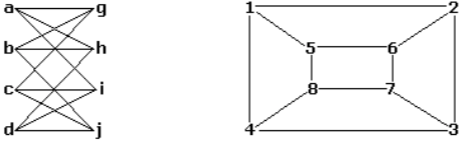
\includegraphics{pic1.png}
\end{center}

Возможным однозначным соответствием, показывающим, что эти два графа
изоморфны, является \t{\{a--1, b--6, c--8, d--3, g--5, h--2, i--4, j--7\}},
хотя существуют и другие подобные соответствия.

Подграфом графа $G$ называется граф, множества вершин и рёбер которого
являются подмножествами множеств вершин и ребер графа $G$.
Заметьте, что граф $G$ является также и своим подграфом.
На рисунке показаны граф и один из его подграфов:

\begin{center}
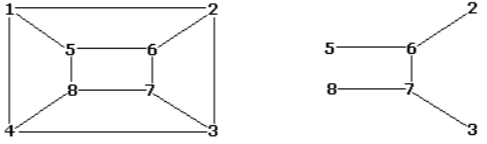
\includegraphics{pic2.png}
\end{center}

Говорят, что граф $G$ содержит другой граф $H$, если существует
хотя бы один подграф $H'$ графа $G$, который изоморфен $H$.
Следующий рисунок показывает граф $G$, который содержит граф $H$.

\begin{center}
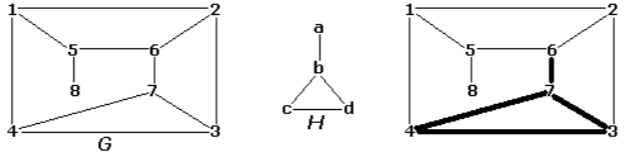
\includegraphics[scale=0.7]{pic3.png}
\end{center}

По двум заданным неориентированным графам $G$ и $H$ постройте подграф $G'$
графа $G$ такой, что:
\begin{itemize}
\item количество вершин в графах $G$ и $G'$ одинаково;
\item $H$ не содержится в $G'$.
\end{itemize}
Естественно, может быть много подграфов графа $G'$
с перечисленными свойствами.
Постройте подграф с как можно большим количеством рёбер.
